\documentclass{article}

\usepackage{csquotes}
\usepackage{graphicx}
\usepackage[margin=2.5cm]{geometry}
\newcounter{boardcounter}
\setcounter{boardcounter}{0}
%This command fills in frame numbers and two blank lines for annotations.
\newcommand{\Annotate}{\stepcounter{boardcounter}[\arabic{boardcounter}]\vspace{\baselineskip}
\rule{\linewidth}{1pt}\\
\rule{\linewidth}{1pt}
\vspace{2\baselineskip}
\vfill
}

\usepackage{xltxtra} % Loads fontspec, xunicode, metalogo, fxltx2e, and some extra customizations for XeLaTeX
%\defaultfontfeatures{Mapping=tex-text} % to support TeX conventions like ``---''
\defaultfontfeatures{Mapping=tex-text}
\setmainfont{Cambria}

%Toggle to switch between languages
%\newcommand\Bislama[1]{#1}
\newcommand\Bislama[1]{}
\newcommand\English[1]{#1}
%\newcommand\English[1]{}
%\newcommand\Daakaka[1]{#1}
\newcommand\Daakaka[1]{}

\begin{document}
\center 
{\huge \Bislama{Fatfat pig}\English{}Bigipigi Ḏamburru} 
\vfill

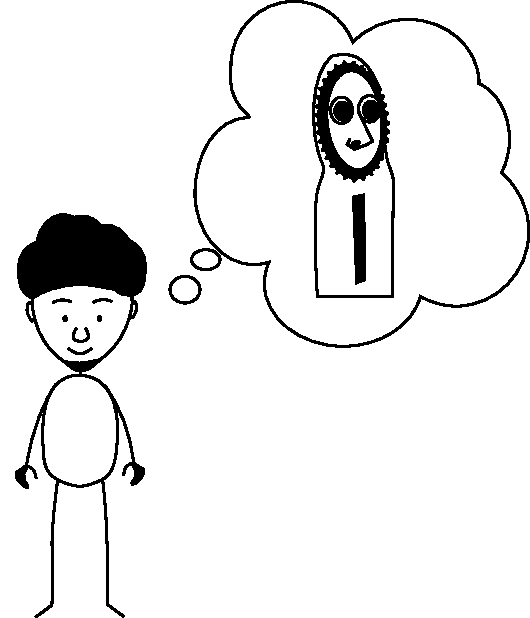
\includegraphics[scale=.7]{StoryboardsFatPig01}

\Bislama{Hemia Denyul. Hemi gat tingting blong mekem wan kastom blong hem.}
\English{This is Denyul. He wants to do a bungguḻ.}
\Daakaka{Denyul mwe pwer te ma ka we poo yan myage.}

\Annotate

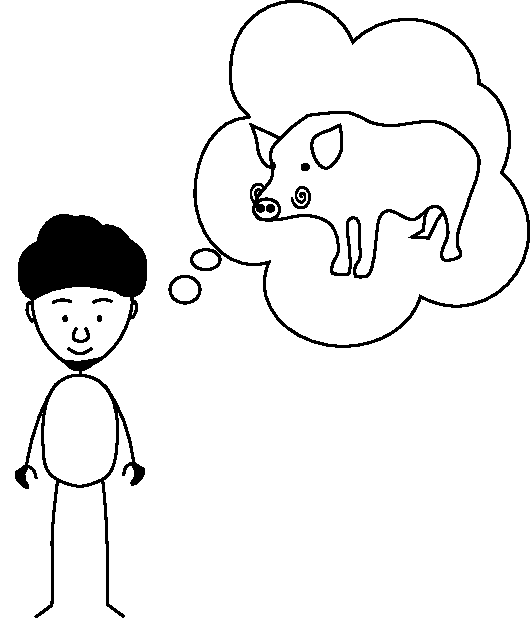
\includegraphics[scale=.7]{StoryboardsFatPig02.pdf}

\Bislama{Blong mekem kastom ia, hemi nidim pig. }
\English{In order to do this, he needs a pig.}
\Daakaka{Te ma dimyane barar swa na luwuon ma ta a towan mwe saa.}

\Annotate

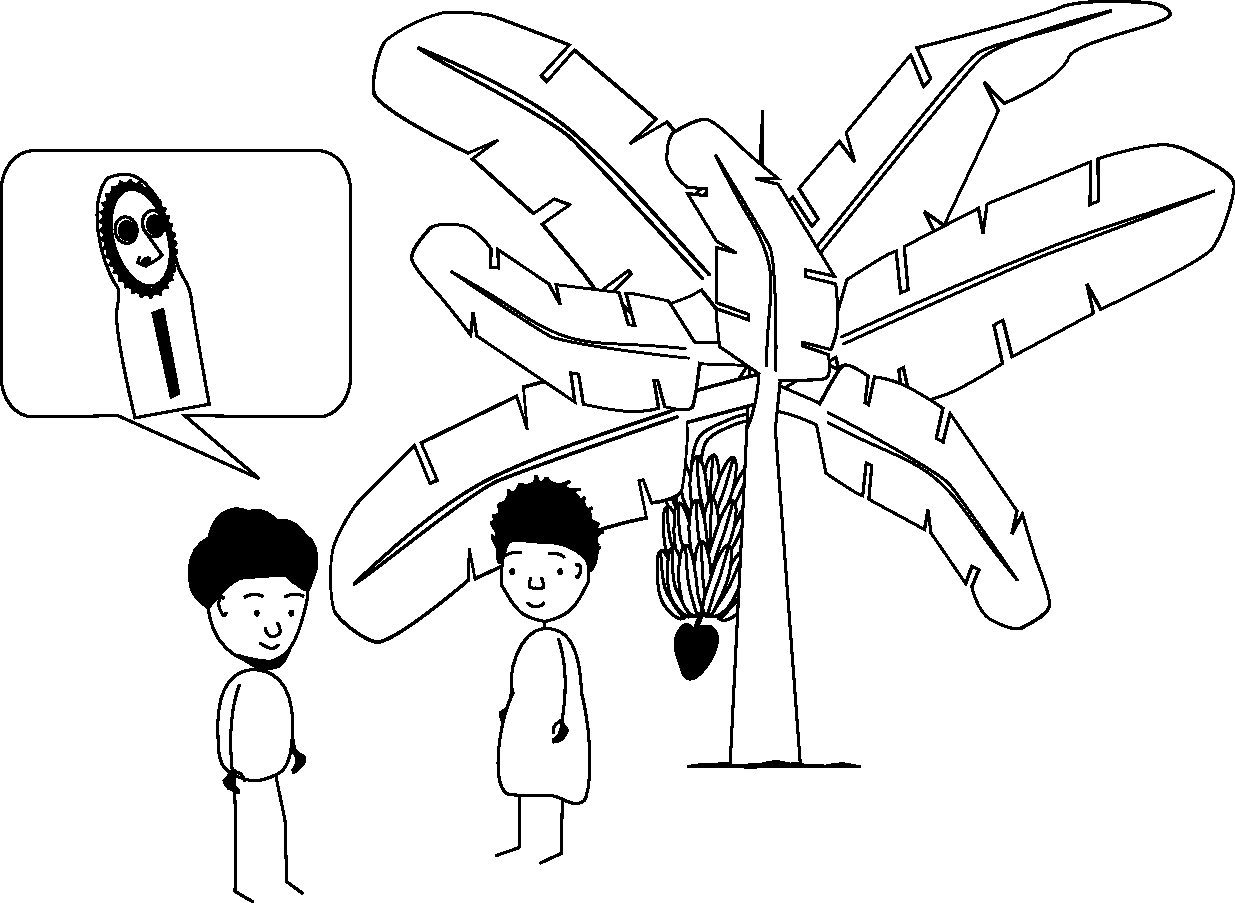
\includegraphics[scale=.55]{StoryboardsFatPig03.pdf}

\Bislama{Ale hemi go luk wan anti blong hem. Denyul hemi se: \enquote{Mi wantem mekem wan kastom blong mi.}}
\English{He goes to see a ŋaṉḏi of his. Denyul says: \enquote{I want to do a custom ceremony.}}
\Daakaka{Mwe vyan te esi san no te ma ka: no, nam dimyane ka nap poo yan myage.}

\Annotate

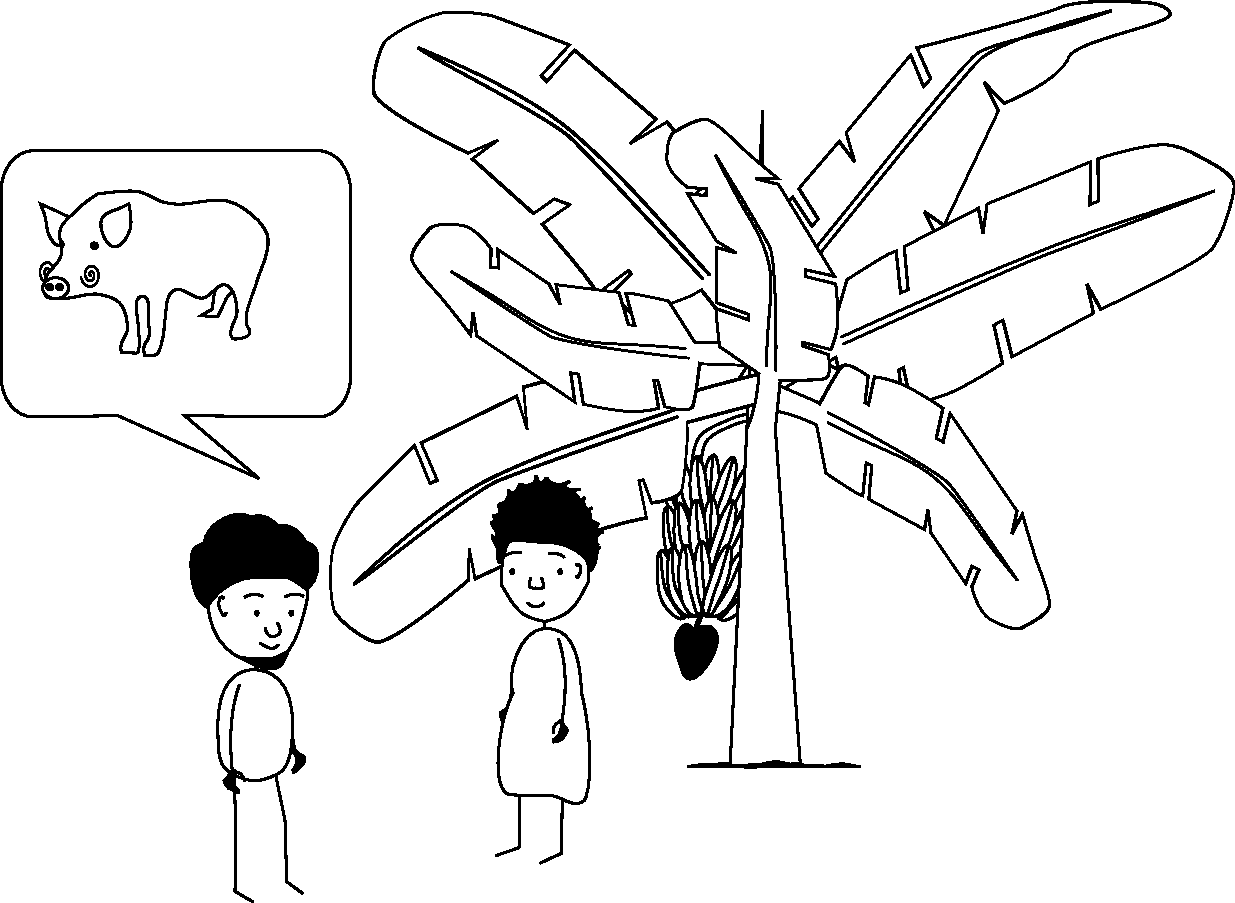
\includegraphics[scale=.55]{StoryboardsFatPig04.pdf}

\Bislama{Ale mi stap lukaotem wan pig.}
\English{So I'm looking for a pig.}
\Daakaka{Nam dimyane barar tuswa.}

\Annotate

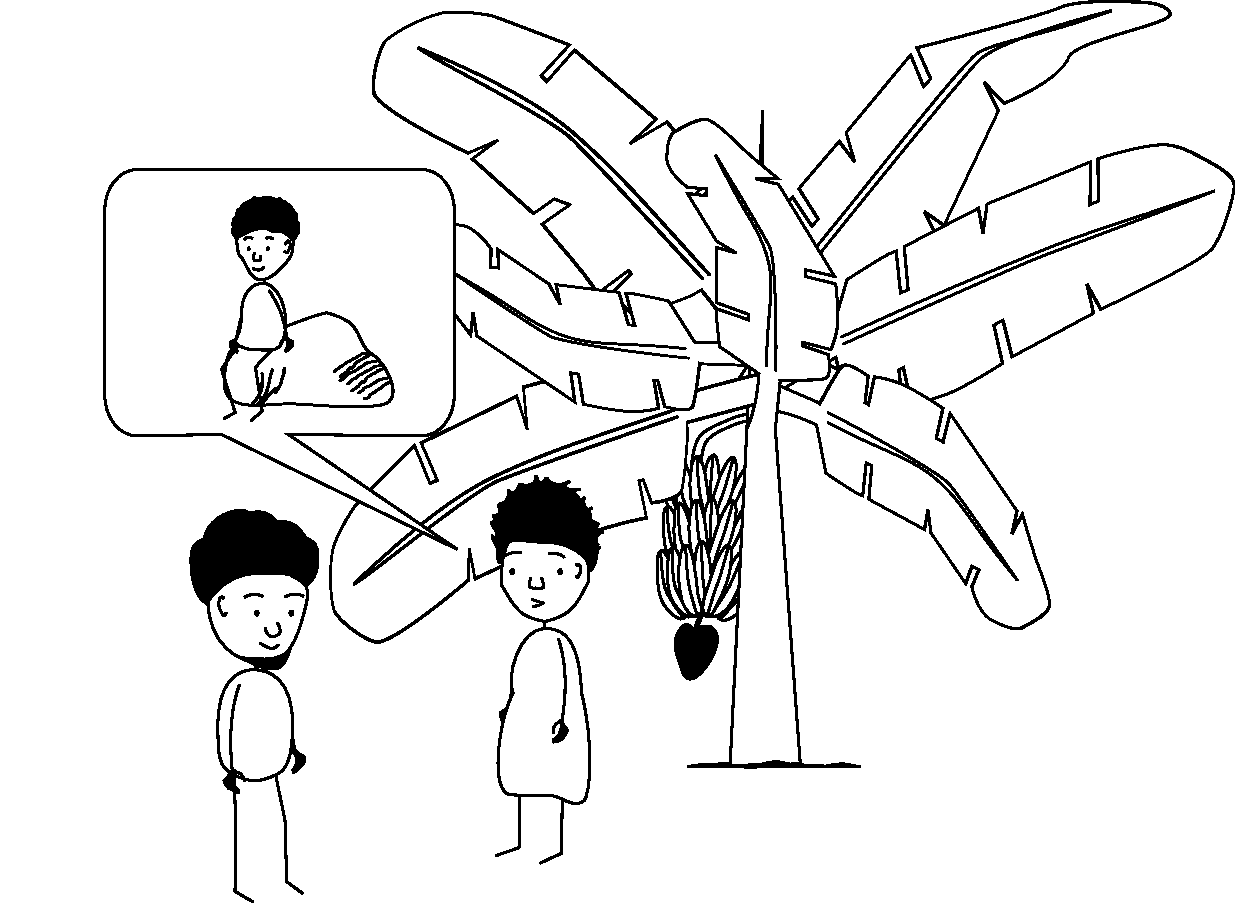
\includegraphics[scale=.6]{StoryboardsFatPig05.pdf}

\Bislama{Ale anti hemi se: \enquote{Bae yu go luk anggel blong yu long narasaed krik.}}
\English{So his ŋaṉḏi says: \enquote{Go visit your ŋapipi on the other side of the river.}}
\Daakaka{Te san no ma ka ko vyan esi sam syuk.}

\Annotate

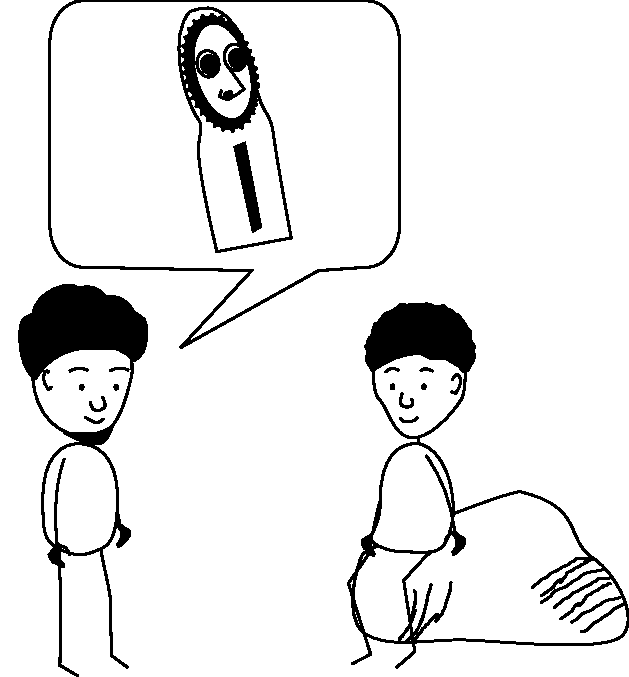
\includegraphics[scale=.7]{StoryboardsFatPig06.pdf}

\Bislama{Afta Denyul hemi go luk angel blong hem. Hemi se: \enquote{Mi wantem mekem wan kastom blong mi.}}
\English{Then Denyul goes to see his uncle. He says: \enquote{I would like to lead a buŋguḻ.}}
\Daakaka{Te mwe vyan esi san syuk, ma ka: syuk, nam ka nap poo yan myage.}

\Annotate

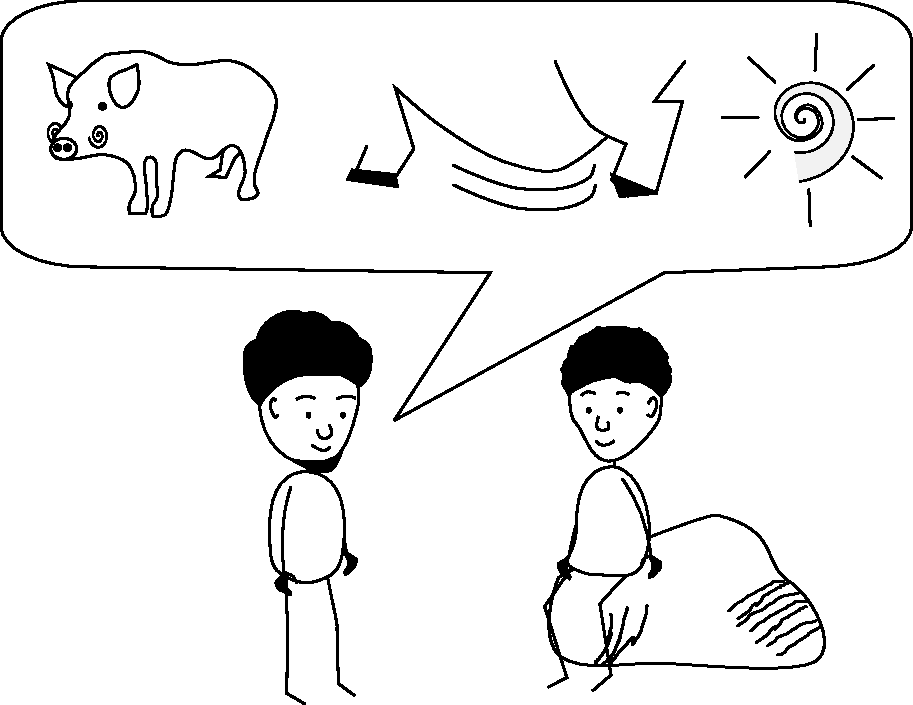
\includegraphics[scale=.7]{StoryboardsFatPig07.pdf}

\Bislama{Ale mi stap lukaotem wan pig we bel i hang i go daon mo tut blong hem i bigwan we i bigwan.}
\English{So I'm looking for a pig which has a fat belly and whose tusks are really long.}
\Daakaka{Nam dimyane barar tuswa na luwuon ma ta a towan mwe saa.}

\Annotate

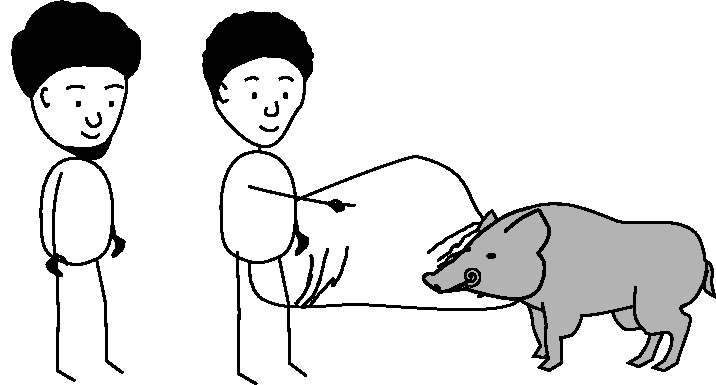
\includegraphics[scale=.7]{StoryboardsFatPig08.pdf}

\Bislama{Afta, anggel ia hemi poentem wan pig hemi se: \enquote{Pig blong mi i stap. I fatfat gud. Mi save givim hem long yu bae yu mekem kastom blong yu.}}
\English{Then his ŋapipi points at a pig and says: \enquote{I have a pig. It is very fat. I can give it to you for your bungguḻ.}}
\Daakaka{Te san syuk mwe sengane barar swa na myorane san nyurnyuran.}

\Annotate
\pagebreak

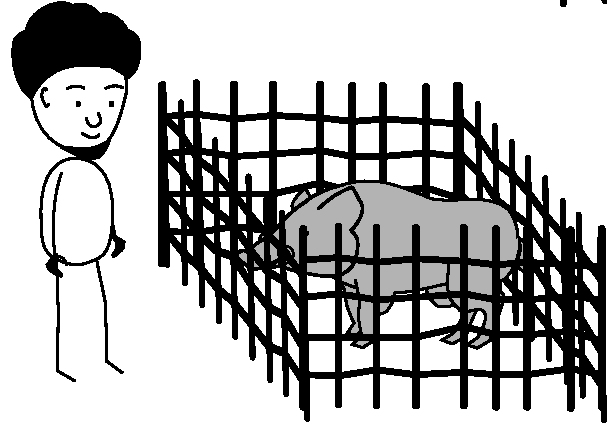
\includegraphics[scale=.6]{StoryboardsFatPig09.pdf}

\Bislama{Ale Denyul hemi tekem pig i go long haos ale putum pig i go long fenis.}
\English{So Denyul takes the pig home and puts it in a pen.}
\Daakaka{Liye barar te vyan te lingi yen biyep.}

\Annotate

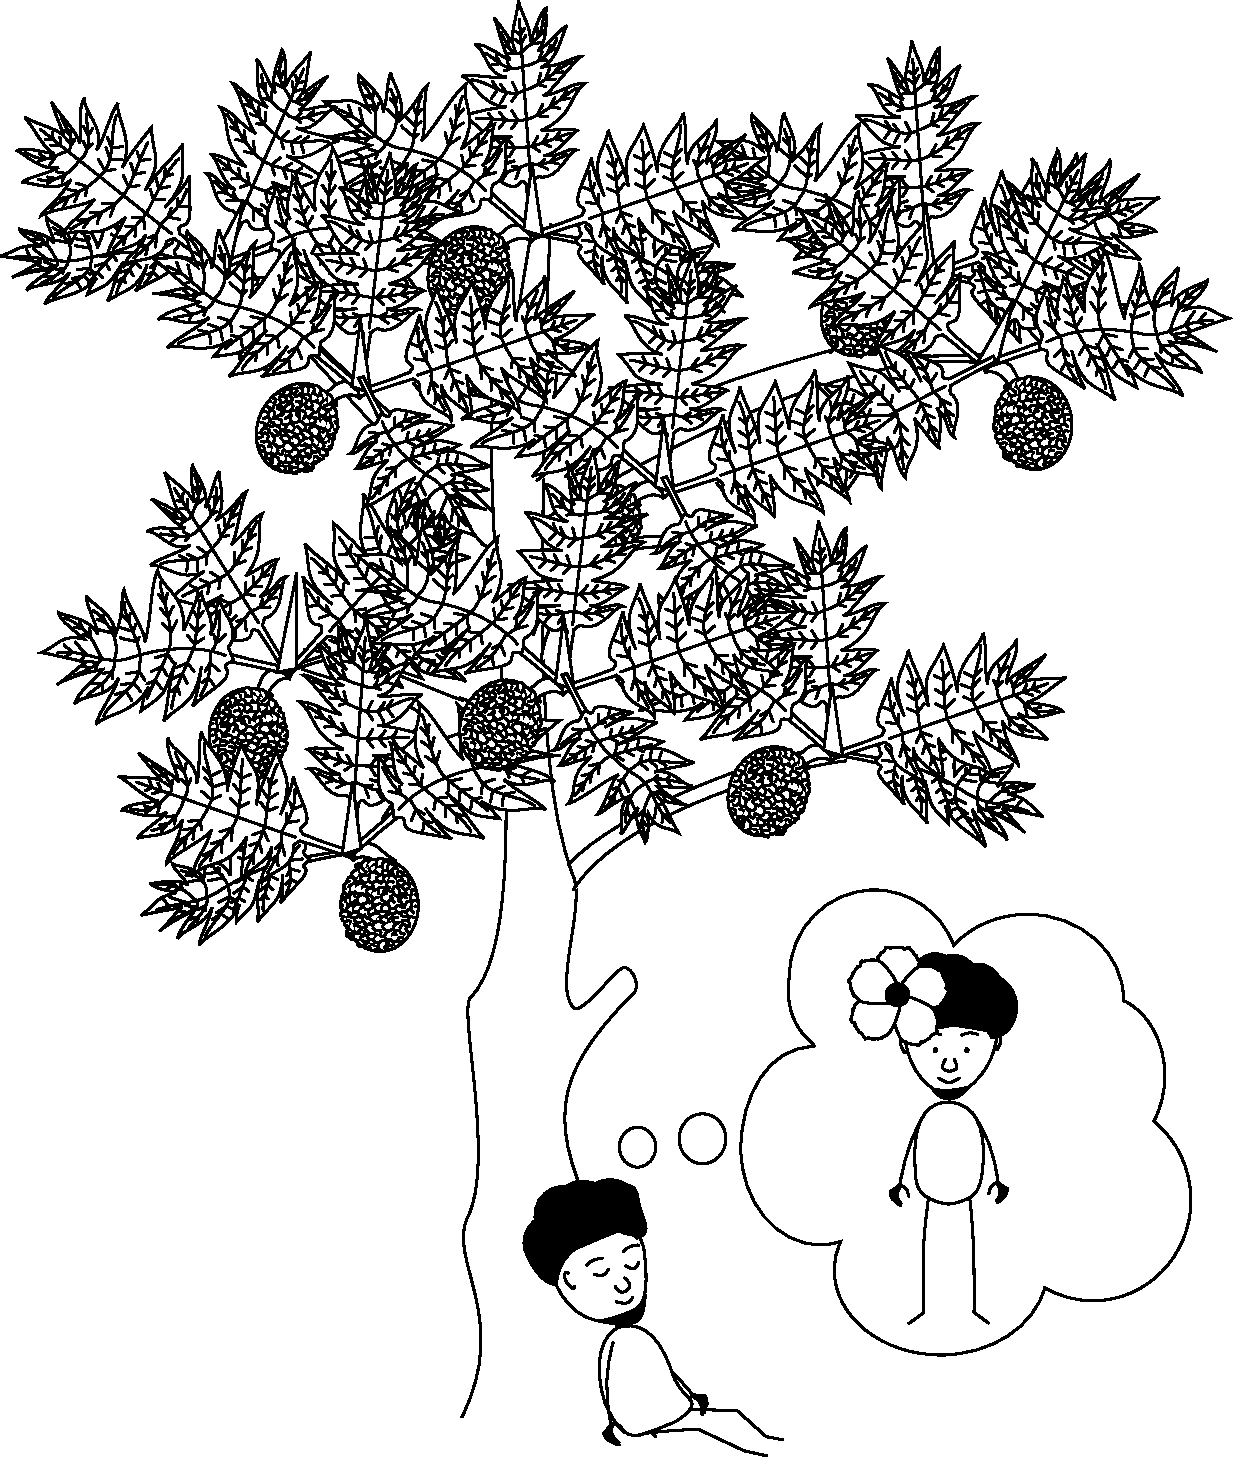
\includegraphics[scale=.5]{StoryboardsFatPig10.pdf}

\Bislama{Afta, hemi go spel, ale silip. Hemi stap drim se bae hemi wan bigman.}
\English{Then he goes to rest and falls asleep. He dreams about being a \textit{buŋgawa}.}
\Daakaka{Ma ongane bip mermer, te vyan pwer te nyurnyurane ka we me yaapu swa wo towo.}

\Annotate

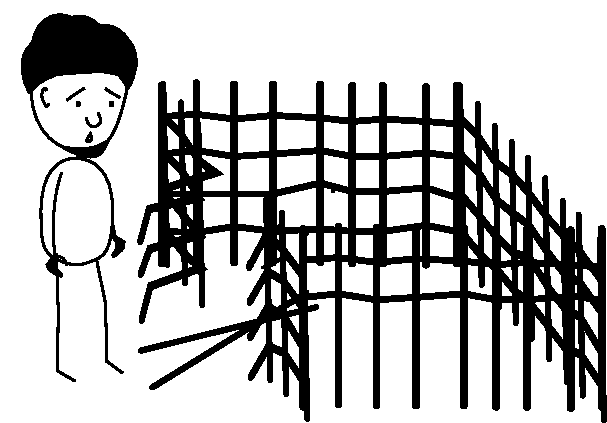
\includegraphics[scale=.6]{StoryboardsFatPig11.pdf}

\Bislama{Be taem hemi go bak long fanis, hemi luk se pig hemi bin brekem fanis ale ron i go.}
\English{But when he goes back to the pen, he sees that the pig has escaped.}
\Daakaka{Mwe tavya vyan te esi barar te barar mu tu te yaase biyep.}

\Annotate

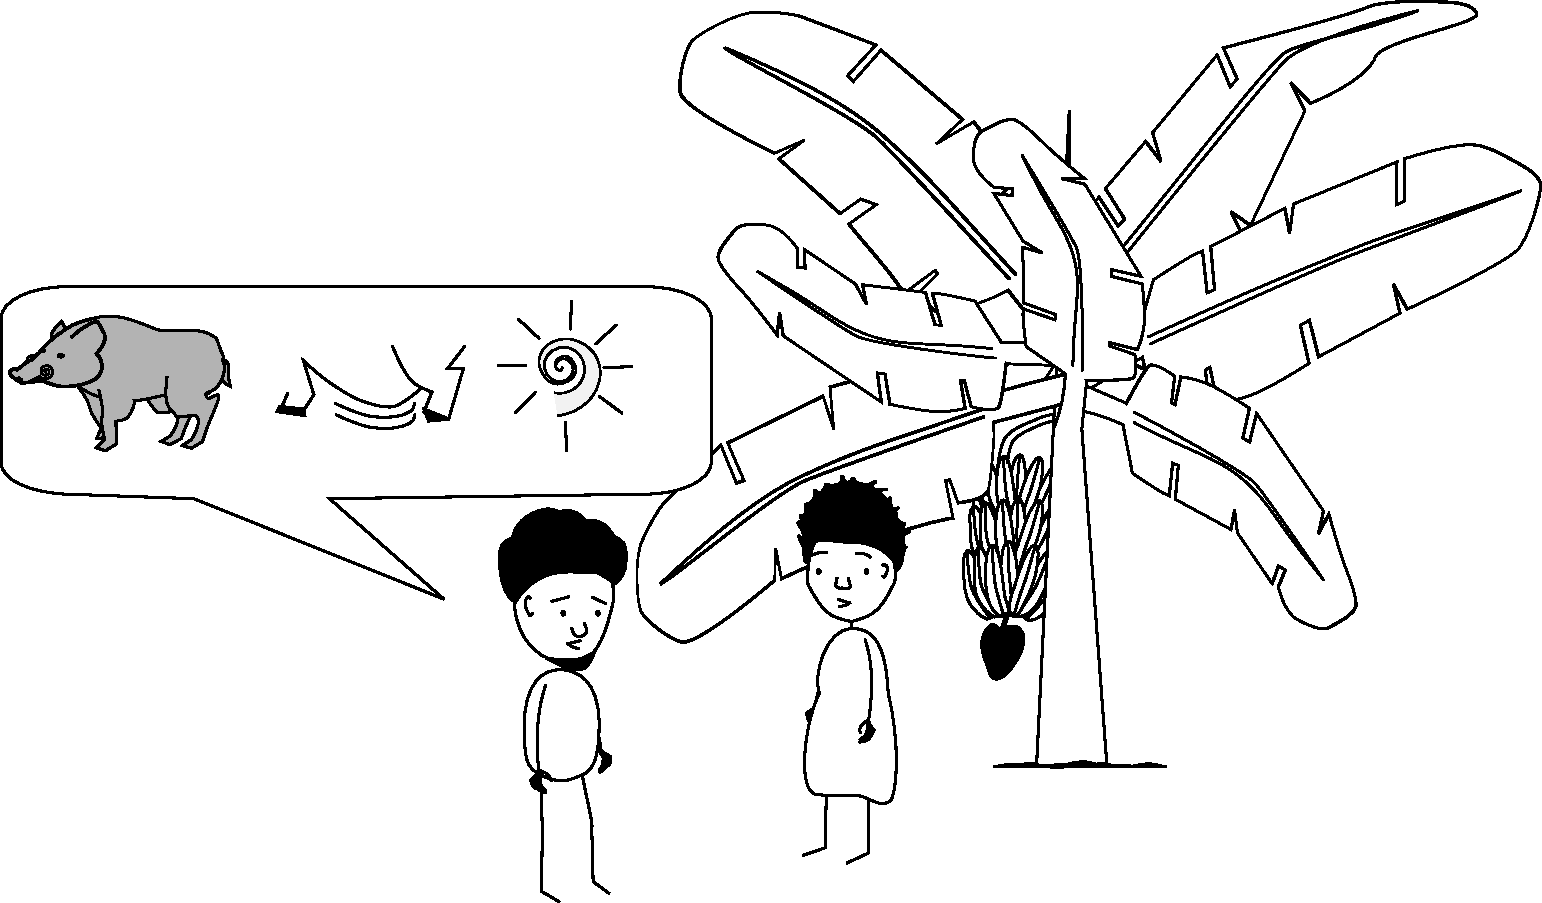
\includegraphics[scale=.7]{StoryboardsFatPig12.pdf}
\Bislama{Ale Denyul hemi go bak long anti blong hem, hemi se: \enquote{Mi stap lukaotem wan pig we bel blong hem i hang mo tut blong hem i bigwan we i bigwan.}}
\English{So Denyul goes back to his ŋaṉḏi and says: \enquote{I'm looking for a pig which is very fat and whose tusks are very long.}}
\Daakaka{Te mwe vyan te esi san no, te ma ka: ko to esi barar swa, luwuon mwe ta, towan mwe saa?}

\Annotate

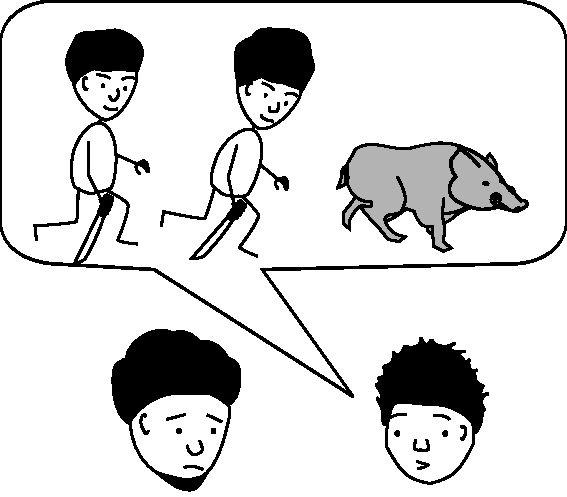
\includegraphics[scale=.7]{StoryboardsFatPig13.pdf}

\Bislama{Anti hemi se: \enquote{Tufala brata blong yu tufala i bin ronem wan pig.}}
\English{His aunt says: \enquote{Two cousins of yours have hunted a pig.}}
\Daakaka{Te san no ma ka: Nam esi sam bivian nya, yem ote barar vyan ate.}

\Annotate

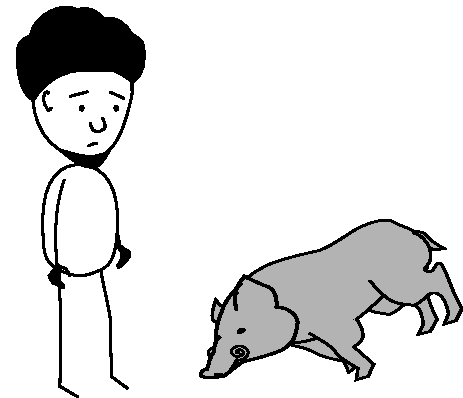
\includegraphics[scale=.7]{StoryboardsFatPig14.pdf}

\Bislama{Ale Denyul hemi go lukluk pig ia, i faenem se i pig blong hem nomo nao we tufala i bin ronem.}
\English{When Denyul goes to look at the dead pig, he sees that it is the one he borrowed.}
\Daakaka{Mwe vyan te esi, an barar yem tyuveni.}

\Annotate

\pagebreak

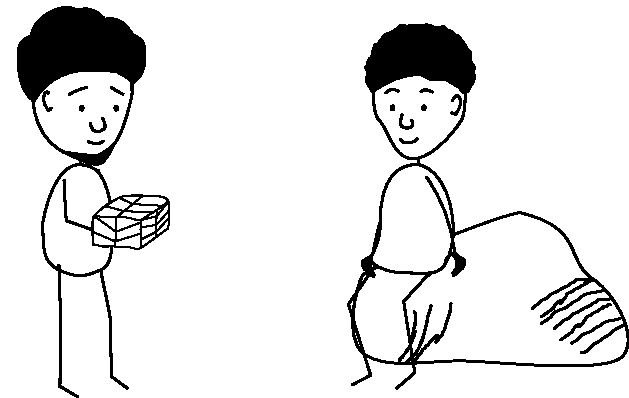
\includegraphics[scale=.7]{StoryboardsFatPig15.pdf}

\Bislama{Denyul hemi sad. Hemi tekem wan pis mit mo rapem long lif blong bae hemi tekem igo long anggel blong hem.}
\English{Denyul is sad. He takes a piece of the pig's meat and wraps it in leaves. Then he takes it to his ŋapipi.}
\Daakaka{Ma sye mur swa vyan te sengane myane san syuk.}

\Annotate

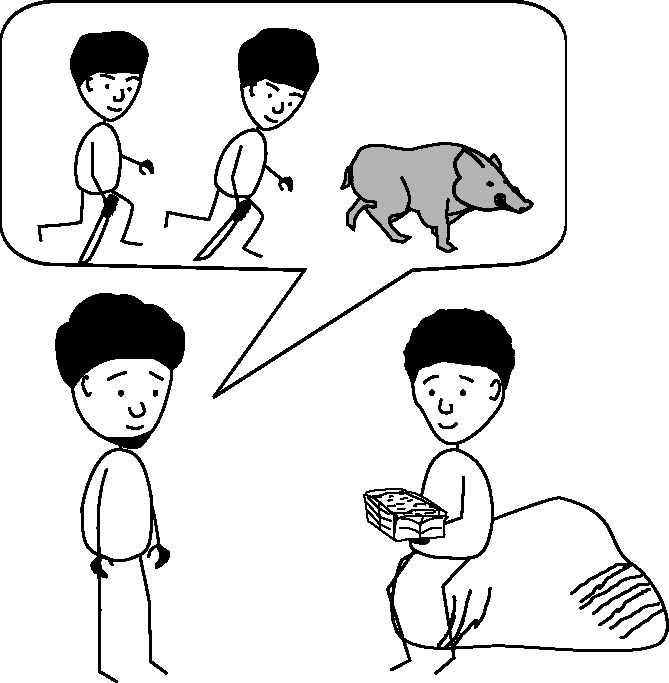
\includegraphics[scale=.7]{StoryboardsFatPig16.pdf}

\Bislama{Anggel hemi tekem mit, hemi talem tankyu long Denyul. Denyul hemi se: \enquote{Mi sori tumas, anggel. Mit ia hemi blong pig blong yu. Ol brata blong mi oli bin ronem.}}
\English{His uncle receives the meat, he thanks Denyul. Denyul says: \enquote{I am very sorry, uncle. This meat is from your pig. My cousins have hunted and killed it.}}
\Daakaka{Sok bivian nya yem tiye barar na kom sengane myane nye.}

\Annotate

\pagebreak

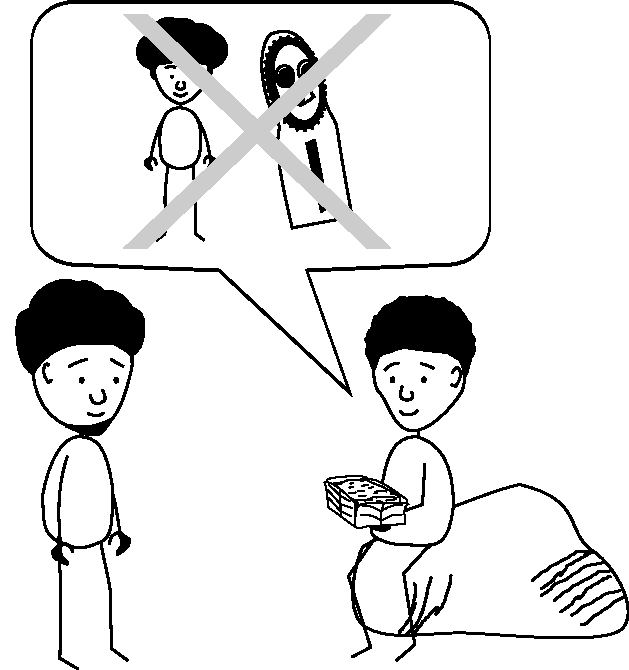
\includegraphics[scale=.7]{StoryboardsFatPig17.pdf}

\Bislama{Anggel hemi se: \enquote{Ating yu no redi blong mekem kastom blong yu yet.}}
\English{His ŋapipi just says: \enquote{I think you are not yet ready to do a buŋguḻ.}}
\Daakaka{Te san syuk ma ka: to wet wese ka kon wet poo yan myage.}

\Annotate

\end{document}